% template adapted from https://github.com/jgm/pandoc-templates/blob/master/default.latex
%%%%%%%%%%%%%%%%%%%%%%%%%%%%%%%%%%%%%%%%%%%%%%%%%%%%%%%%%%%%%%%%%%%%%%%%%%%%%%%%%%%%%%%%%

% Options for packages loaded elsewhere
\PassOptionsToPackage{unicode=true}{hyperref}
\PassOptionsToPackage{hyphens}{url}
  \PassOptionsToPackage{dvipsnames,svgnames*,x11names*}{xcolor}


\documentclass[
  11pt,
  french,
  A4paper,
  extrafontsizes,onecolumn,openright
  ]{memoir}

% Font family: lmodern by default
  \usepackage{lmodern}

% Double (or whatever) spacing

\usepackage{amssymb, amsmath}
\usepackage{ifxetex,ifluatex}
\usepackage{fixltx2e} % provides \textsubscript

% mathspec: arbitrary math fonts
  \usepackage{unicode-math}
\defaultfontfeatures{Ligatures=TeX,Scale=MatchLowercase}

% More font families
% Main font
% Specific sanserif font
% Specific monotype font
% Specific math font
% Chinese, Japanese, Corean fonts

% Use upquote if available, for straight quotes in verbatim environments
\IfFileExists{upquote.sty}{\usepackage{upquote}}{}
% Use microtype if available
\IfFileExists{microtype.sty}{%
\usepackage[]{microtype}
\UseMicrotypeSet[protrusion]{basicmath} % disable protrusion for tt fonts
}{}

% Verbatim in note

\usepackage{xcolor}

\usepackage{hyperref}
\hypersetup{
            pdftitle={Trajectoires de biodiversité en forêt tropicale exploitée},
            pdfauthor={Ariane Mirabel},
            pdfkeywords={Biodiversity, Neotropical forests, Perturbation, Communities Ecology, Dynamic trajectories, Resilience},
            colorlinks=true,
            linkcolor=Maroon,
            citecolor=Blue,
            urlcolor=Blue,
            breaklinks=true}

% Don't use monospace font for urls
\urlstyle{same}


% Geometry package

% Listings package


\usepackage{color}
\usepackage{fancyvrb}
\newcommand{\VerbBar}{|}
\newcommand{\VERB}{\Verb[commandchars=\\\{\}]}
\DefineVerbatimEnvironment{Highlighting}{Verbatim}{commandchars=\\\{\}}
% Add ',fontsize=\small' for more characters per line
\usepackage{framed}
\definecolor{shadecolor}{RGB}{248,248,248}
\newenvironment{Shaded}{\begin{snugshade}}{\end{snugshade}}
\newcommand{\KeywordTok}[1]{\textcolor[rgb]{0.13,0.29,0.53}{\textbf{#1}}}
\newcommand{\DataTypeTok}[1]{\textcolor[rgb]{0.13,0.29,0.53}{#1}}
\newcommand{\DecValTok}[1]{\textcolor[rgb]{0.00,0.00,0.81}{#1}}
\newcommand{\BaseNTok}[1]{\textcolor[rgb]{0.00,0.00,0.81}{#1}}
\newcommand{\FloatTok}[1]{\textcolor[rgb]{0.00,0.00,0.81}{#1}}
\newcommand{\ConstantTok}[1]{\textcolor[rgb]{0.00,0.00,0.00}{#1}}
\newcommand{\CharTok}[1]{\textcolor[rgb]{0.31,0.60,0.02}{#1}}
\newcommand{\SpecialCharTok}[1]{\textcolor[rgb]{0.00,0.00,0.00}{#1}}
\newcommand{\StringTok}[1]{\textcolor[rgb]{0.31,0.60,0.02}{#1}}
\newcommand{\VerbatimStringTok}[1]{\textcolor[rgb]{0.31,0.60,0.02}{#1}}
\newcommand{\SpecialStringTok}[1]{\textcolor[rgb]{0.31,0.60,0.02}{#1}}
\newcommand{\ImportTok}[1]{#1}
\newcommand{\CommentTok}[1]{\textcolor[rgb]{0.56,0.35,0.01}{\textit{#1}}}
\newcommand{\DocumentationTok}[1]{\textcolor[rgb]{0.56,0.35,0.01}{\textbf{\textit{#1}}}}
\newcommand{\AnnotationTok}[1]{\textcolor[rgb]{0.56,0.35,0.01}{\textbf{\textit{#1}}}}
\newcommand{\CommentVarTok}[1]{\textcolor[rgb]{0.56,0.35,0.01}{\textbf{\textit{#1}}}}
\newcommand{\OtherTok}[1]{\textcolor[rgb]{0.56,0.35,0.01}{#1}}
\newcommand{\FunctionTok}[1]{\textcolor[rgb]{0.00,0.00,0.00}{#1}}
\newcommand{\VariableTok}[1]{\textcolor[rgb]{0.00,0.00,0.00}{#1}}
\newcommand{\ControlFlowTok}[1]{\textcolor[rgb]{0.13,0.29,0.53}{\textbf{#1}}}
\newcommand{\OperatorTok}[1]{\textcolor[rgb]{0.81,0.36,0.00}{\textbf{#1}}}
\newcommand{\BuiltInTok}[1]{#1}
\newcommand{\ExtensionTok}[1]{#1}
\newcommand{\PreprocessorTok}[1]{\textcolor[rgb]{0.56,0.35,0.01}{\textit{#1}}}
\newcommand{\AttributeTok}[1]{\textcolor[rgb]{0.77,0.63,0.00}{#1}}
\newcommand{\RegionMarkerTok}[1]{#1}
\newcommand{\InformationTok}[1]{\textcolor[rgb]{0.56,0.35,0.01}{\textbf{\textit{#1}}}}
\newcommand{\WarningTok}[1]{\textcolor[rgb]{0.56,0.35,0.01}{\textbf{\textit{#1}}}}
\newcommand{\AlertTok}[1]{\textcolor[rgb]{0.94,0.16,0.16}{#1}}
\newcommand{\ErrorTok}[1]{\textcolor[rgb]{0.64,0.00,0.00}{\textbf{#1}}}
\newcommand{\NormalTok}[1]{#1}

% Tables
  \usepackage{longtable,booktabs}
  % Fix footnotes in tables (requires footnote package)
  \IfFileExists{footnote.sty}{\usepackage{footnote}\makesavenoteenv{longtable}}{}

% Graphics
  \usepackage{graphicx,grffile}
  \graphicspath{{images/}}
  \makeatletter
  \def\maxwidth{\ifdim\Gin@nat@width>\linewidth\linewidth\else\Gin@nat@width\fi}
  \def\maxheight{\ifdim\Gin@nat@height>\textheight\textheight\else\Gin@nat@height\fi}
  \makeatother
  % Scale images if necessary, so that they will not overflow the page
  % margins by default, and it is still possible to overwrite the defaults
  % using explicit options in \includegraphics[width, height, ...]{}
  \setkeys{Gin}{width=\maxwidth,height=\maxheight,keepaspectratio}



\setlength{\emergencystretch}{3em}  % prevent overfull lines
\providecommand{\tightlist}{%
  \setlength{\itemsep}{0pt}\setlength{\parskip}{0pt}}

  \setcounter{secnumdepth}{5}

% set default figure placement to htbp
\makeatletter
\def\fps@figure{htbp}
\makeatother

% Include headers (preamble.tex) here
%%% Complete the preamble of the LaTeX template
%%%------------------------------------------------------------------------------

%%% PACKAGES 
\usepackage{lipsum} % Dummy text.

\usepackage{enumitem}

  % load polyglossia as late as possible as it *could* call bidi if RTL lang (e.g. Hebrew or Arabic)
  \usepackage{polyglossia}
  \setmainlanguage[]{french}
  \setotherlanguage[variant=american]{english}
  \setotherlanguage[variant=british]{english}
  \setotherlanguage[]{french}




\usepackage[style=authoryear,backend=bibtex,citestyle=authoryear,isbn=false,backref=true,giveninits=true,uniquename=init,maxcitenames=2,maxbibnames=150,sorting=nyt,sortcites=false]{biblatex}
\addbibresource{packages.bib}
\addbibresource{01ref-IntroG.bib}
\addbibresource{02ref-chap2Incert.bib}

% Specific commands for EcoFoG style. Must come after biblatex.
\usepackage{latex/BookTemplate}


% Title, author, etc. from YAML to LaTeX
%%%%%%%%%%%%%%%%%%%%%%%%%%%%%%%%%%%%%%%%%%%%%%%%%%%%%%%%%%

\title{Trajectoires de biodiversité en forêt tropicale exploitée}


\author{Ariane Mirabel}


\date{2018-06-18}


% Main title page with filigrane
%%%%%%%%%%%%%%%%%%%%%%%%%%%%%%%%%%%%%%%%%%%%%%%%%%%%%%%%%%

\newcommand{\MainTitlePage}[1][]{
	\SmallMargins % Margins
	\pagestyle{empty} % No header/footer
	~\\ % Print a character or the page will not exist
	\begin{textblock}{2}(30,10)
		\rule{1pt}{\paperheight-20mm}
	\end{textblock}
	\begin{textblock}{140}(50, 45)
		\flushright
		\begin{Spacing}{3}
			{\fontfamily{qtm}\selectfont\fontsize{45}{45}\selectfont \textsc{\thetitle}}
		\end{Spacing}
	\end{textblock}
	\begin{textblock}{140}(50, 125)
		\flushright
		{\fontfamily{qtm}\Large \theauthor}
	\end{textblock}
	\begin{textblock}{120}[1, 1](225, 297)
		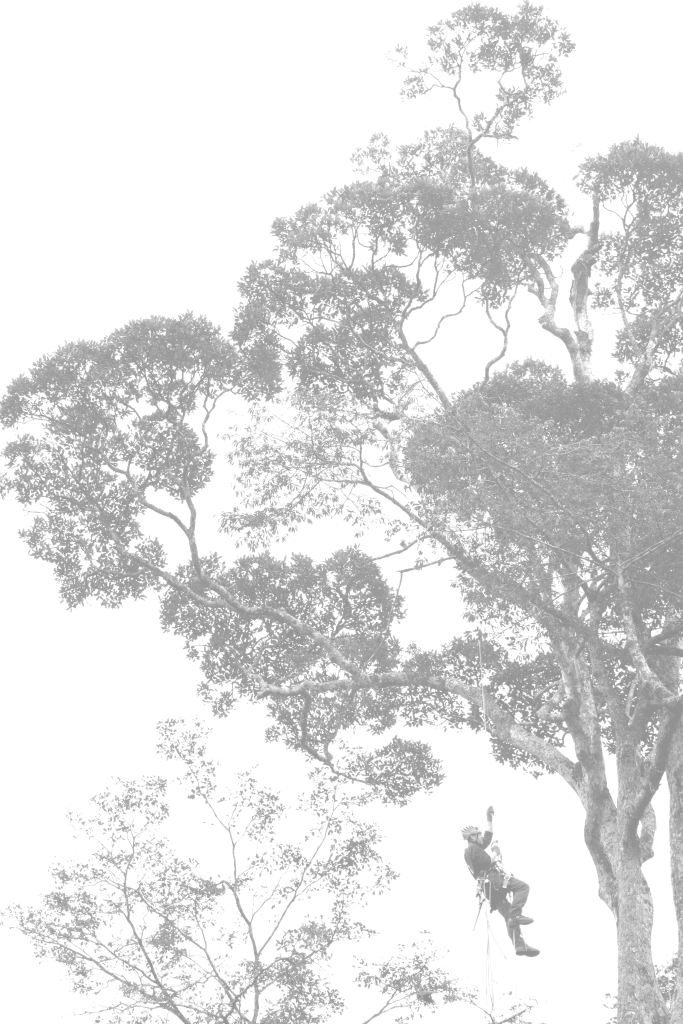
\includegraphics[width=10cm]{Filigrane}
	 \end{textblock}
	\begin{textblock}{140}[0, 1](50, 262)
		\normalfont	Version: \thedate
	\end{textblock}
	\newpage
	~\\ % Print a character or the page will not exist
	\begin{textblock}{140}(40, 40)
		#1
	\end{textblock}
	\begin{textblock}{140}[0,1](40, 270)
		\centering
    \includegraphics[width=5cm]{Logo-Lab}\\ \bigskip
		UMR \'Ecologie des forêts de Guyane\\
		\url{http://www.ecofog.gf}\\[3\baselineskip]
		Les opinions émises par les auteurs sont personnelles et n’engagent ni l’UMR EcoFoG ni ses tutelles.

    \tiny{Photographie en couverture: Hadrien Lalagüe}
	\end{textblock}
	\newpage
}

% PhD / HDR Thesis
%%%%%%%%%%%%%%%%%%%%%%%%%%%%%%%%%%%%%%%%%%%%%%%%%%%%%%%%%%

\usepackage[DocType=PhD, ED=UG, Ets=UG, DIS=ST]{latex/pdgUniv}

\specialty{Ecologie}
\defencedate{1er janvier 2018}
\lab{Ecologie des forets de Guyane}
% ==================
% Setup people like your boss, the jury team and the referees
% - First you need to define how number they will be in each category
%   It is done with the commands \nboss{n}, \nreferee{n} and \njudge{n}.
%   You can define more people in each category than the number given
%   but only the first "\npeople" will be print.
% - Then use the command \makesomeone{<category>}{<number>}{<name>}{<status>}{<other>}
%   where:
%     <category> should be select in ['boss', 'referee', 'judge']
%     <number>   is the rank for printing the person.
%                Only number <= "\npeople" will be printed
%     <name>     First name and las name of the people
%     <status>   Is (s)he a "charg\'e de recher" ou un "professeur d'universit\'e"...
%     <other>    What ever string you want to add (laboratory, jury member place...).
\njudge{7}
\makesomeone{judge}{1}{Prenom NomJury1}{Professeur d'Universite}{Membre du Jury}
\makesomeone{judge}{2}{Prenom NomJury2}{Professeur d'Universite}{Membre du Jury}
\makesomeone{judge}{3}{Prenom NomJury3}{Professeur d'Universite}{Membre du Jury}
\makesomeone{judge}{4}{Prenom NomJury4}{Professeur d'Universite}{Membre du Jury}
\makesomeone{judge}{5}{Prenom NomJury5}{Professeur d'Universite}{Membre du Jury}
\makesomeone{judge}{6}{Prenom NomJury6}{Professeur d'Universite}{Membre du Jury}
\makesomeone{judge}{7}{Prenom NomJury7}{Professeur d'Universite}{Membre du Jury}



% End of preamble
%%%%%%%%%%%%%%%%%%%%%%%%%%%%%%%%%%%%%%%%%%%%%%%%%%%%%%%%%%


\begin{document}
\frontmatter

% Title page
%%%%%%%%%%%%%%%%%%%%%%%%%%%%%%%%%%%%%%%%%%%%%%%%%%%%%%%%%%


\makeflyleaf




% Before Body
%%%%%%%%%%%%%%%%%%%%%%%%%%%%%%%%%%%%%%%%%%%%%%%%%%%%%%%%%%




% Contents
%%%%%%%%%%%%%%%%%%%%%%%%%%%%%%%%%%%%%%%%%%%%%%%%%%%%%%%%%%

\LargeMargins
{
\hypersetup{linkcolor=}
\setcounter{tocdepth}{3}
\tableofcontents
}


% Body
%%%%%%%%%%%%%%%%%%%%%%%%%%%%%%%%%%%%%%%%%%%%%%%%%%%%%%%%%%

\LargeMargins
\mainmatter

\chapter{Introduction générale}\label{introduction-generale}

\section{Les forêts tropicales humides, au coeur de l'avenir
planétaire}\label{les-forets-tropicales-humides-au-coeur-de-lavenir-planetaire}

Les forêts couvrent 30\% de la surface terrestre et les nombreux biens
et services environnementaux, économiques et sociaux qu'elles assurent
sont indispensables à l'équilibre planétaire. Elles régulent le climat,
la qualité de l'eau, de l'air et des sols et abritent une diversité
biologique exceptionnelle. Elles subviennent aux besoins alimentaires de
la population mondiale et permettent son développement économique en
tant que source de matières premières, de revenus et d'opportunités de
développement. Enfin, indispensables au bien être des populations, elles
représentent des valeurs historiques, culturelles et patrimoniales
irremplaçables \autocites{FRA2015}{Tilman2014}. Malgré leur importance
les forêts restent extrêmement menacées par les changements climatiques
globaux, le traffic de bois illégal, la déforestation liée aux
changements d'usage des terres et les dégradations et pollutions
environnementales.

\subsection{Des écosystèmes
incontournables}\label{des-ecosystemes-incontournables}

Par ``forêt'' ou ``ecosystème forestier'' on entend les assemblages de
plantes, animaux et microorganismes et leur environnement qui
définissent une unité fonctionnelle dont les arbre sont les composants
essentiels \autocite{FRA2000}. Ces écosystèmes accueillent la diversité
animale et végétale et les taux d'endémismes les plus importants du
globe et sont les régions restées les moins anthropisées ce qui leur
confère de forts enjeux de conservation
\autocites{Myers2000}{Mittermeier2003}.

En entretenant les cycles de l'eau et des nutriments (azote, phosphore,
etc) via leur réseau racinaire, les forêts régulent la fertilité des
sols et les températures et les précipitations locales
\autocites{Malhi2008}{Isbell2017}. Elles sont également des puits de
carbone qui représentent 1.1 ± 0.8 PgC.yr\textsuperscript{--1} et jouent
un rôle majeur dans la régulation des gaz à effet de serre (\emph{GES}),
d'une part en tant que puit de carbone qui compense les émissions de GES
mais également an tant que source potentielle lorsque leur dégradation
libère le carbone stocké dans leur biomasse
\autocites{Pan2011}{Roy2017}.

A l'échelle globale la subsistance de 500 millions de personnes dépend
directement des forêts qui sont une source de biens allant de la
nourriture (par la chasse et la collecte de produits forestiers non
ligneux comestibles), à l'eau, aux matériaux de construction, et à
l'énergie (par l'utilisation du bois de chauffage et de cuisson des
aliments). L'exploitation forestière quant à elle représentait
\textasciitilde{} 1\% du PIB mondial, une part importante de l'emploi et
l'une des principales sources d'énergie en 2011
\autocites{CBDdiversity2011}{FAO2014}.

Enfin, les forêts interconnectées depuis toujours aux populations
humaines sont indispensables à leur bien être et ont une dimension
culturelle, spirituelle et patrimoniale importante.

\subsection{Des écosystèmes menacés, en particulier sous les
tropiques}\label{des-ecosystemes-menaces-en-particulier-sous-les-tropiques}

Bien qu'aussi indispensables qu'irremplaçables, les forêts disparaissent
et sont dégradées à une vitesse croissante: entre 2013 et 2015 leur
surface globale a ainsi diminué de 3\% \autocite{FAO2009}. Les forêts
sont soumises à de fortes pressions anthropiques allant des changements
d'usage des terres, tels que le déboisement pour l'élevage ou
l'agriculture, à l'exploitation du bois légale ou illégale, à la chasse
ou à l'introduction d'espèces invasives. Elles subissent de plus les
changements climatiques globaux qui augmentent la fréquence des
événements extrêmes (sécheresses, incendies, inondations\ldots{})
\autocite{Pachauri2014}.

Ces pressions diverses persistent voire s'accentuentmalgré une prise de
conscience globale entérinée par la conférence des nations unies sur
l'environnement et le développement à Rio en 1992 qui a motivé de
nombreuses politiques de surveillance, de conservation de la
biodiversité et de préservation du fonctionnement des forêts
\autocites{Summit1992}{Schlaepfer2000}{Dirzo2003a}{Morales-Hidalgo2015}.

Ce contexte concerne en particulier les forêts tropicales, pour
lesquelles les menaces sont d'autant plus graves que leur importance au
niveau mondial est grande \autocites{Dirzo2003a}{Hansen2013}. Les
bassins forestiers tropicaux qui représentent 1.3 million d'hectares
sont plus grandes surfaces de forêts anciennes ``primaires'' n'ayant pas
connu de forte perturbation anthropique et accueillent la diversité
biologique la plus élevée au monde \autocites{Gentry1988}{FAO2011}.
Historiquement peu peuplées, ces régions connaissent une croissance
démographique moyenne de près de 1,4\% par an qui entraîne des pressions
anthropiques croissantes de chasse, d'exploitation du bois, de
conversion en terres agricoles et de dégradation en forêts secondaires
\autocite{Asner2009}.

Une attention particulière doit être portée aux zones tropicales pour
mieux comprendre leurs dynamiques et leur fonctionnement, toujours
partiellement méconnus aujourd'hui.

\subsection{La biodiversité: clé du fonctionnement des forêts
tropicales}\label{la-biodiversite-cle-du-fonctionnement-des-forets-tropicales}

La biodiversité n'est pas épargnée par les pressions globales actuelles
et une fraction significative est déjà anéantie et continue de
disparaître irréversiblement, si bien que l'on qualifie déjà cette
érosion croissantede sixième extinction de l'ère moderne
\autocites{Vitousek1997}{Cardinale2012}.

La diversité des arbres, qui sont les éléments essentiels des
écosystèmes forestiers, détermine largement leur fonctionnement et
reflète celle autres groupes floristiques ou faunistiques
\autocite{Guitet2017}. Individuellement d'une part, les espèces ont une
valeur intrinsèque qui constitue le patrimoine naturel global et selon
leurs charactéristiques biologiques peuvent avoir un rôle primordial,
comme c'est le cas pour les espèces \emph{clé de voûte},
\autocites{Jones1994}{Power1996}{Gardner2007}. D'autre part, la
diversité et la composition d'une communauté dans son ensemble définit
la complémentarité entre les individus qui la composent et l'utilisation
et la transformation des ressources. La diversité d'une communauté
détermine les flux d'eau, de nutriments et d'énergie à la base des
processus écosystémiques et donc sa productivité \autocite{Begon2006}.
Une diversité élevée est de plus garante de la stabilité et la
résilience des écosystèmes en palliant l'impact des maladies, des
espèces invasives et des variations environnementales
\autocite{Elmqvist2003}.

On sait aujourd'hui que l'érosion de la biodiversité impacte le
fonctionnement des forêts mais les conséquences précises et la réponse
des écosystèmes dans le contexte actuel de changements globaux restent
mal connus. Pour avoir une comprendre et anticiper le devenir des forêts
dans le contexte actuel il est primordial de déterminer leurs dynamique
et leur réponse aux perturbation dans l'ensemble des aspects de leur
biodiversité.

\section{Les déterminants de la biodiversité: dynamique des communautés
et règles
d'assemblage}\label{les-determinants-de-la-biodiversite-dynamique-des-communautes-et-regles-dassemblage}

L'enjeu dans le contexte actuel est de prédire la réponse des
communautés aux perturbations en termes de diversité et de composition
et l'impact de ces changements sur leur fonctionnement des écosystèmes.
Comprendre et anticiper la réponse des peuplements revient à identifier
les processus écologiques qui régissent la dynamique des communautés et
qui déterminent la composition et la structure de la communauté à venir.

\subsection{Les règles d'assemblage des
espèces}\label{les-regles-dassemblage-des-especes}

La question fondamentale de l'écologie est de comprendre les processus
impliqués dans l'assemblage et la coexistence des espèces en
communautés. Plusieurs hypothèses sont débattues aujourd'hui, invoquant
soit des processus déterministes qui sélectionnent les espèces selon
leurs aptitudes dans l'environnement biotique et abiotique considéré
\autocite{Molino2001}, soit des processus stochastiques relevant de la
théorie neutre qui supposent un assemblage dépendant uniquement de
contraintes historiques et de limitation de dispersion ou de croissance
\autocite{Hubbell2001} \ref{fig:AssemblyRules}.

Ce débat sur les processus écologiques responsables de la structuration
des communautés est matérialisé dans le cas des forêts tropicales par la
controverse sur la théorie des perturbations intermédiaires
(\emph{Intermediaite Disturbance Hypothesis, IDH} en anglais). Cette
théorie prédit la prépondérance de processus déterministes d'exclusion
compétitive et de filtrage des espèces qui conduirait à une diversité
maximale pour un régime moyen de perturbations \autocite{Molino2001}. Un
tel régime de perturbations modifierait régulièrement mais non
drastiquement l'environnment et créerait une variabilité constante dans
l'espace et le temps des conditions biotiques (interactions entre
individus) et abiotiques (ensoleillement, température, flux d'eau et de
matière). Cette variabilité permettrait à un large panel d'espèces de
s'installer soit parce que les conditions environnementales leur sont
devenues favorables soit parce qu'elles deviennent plus compétitives
relativement au reste de la communauté
\autocites{Chesson2000alire}{Kariuki2006a}{Berry2008a}. A l'inverse la
théorie neutre suppose que les espèces sont équivalentes et que leur
abondance ne dépend pas de leurs caractéritiques écologiques et
fonctionnelles mais de processus aléatoires de dispersion, de croissance
et de survie qui résultent en un assemblage stochastique des communautés
\autocite{Hubbell2001}. Les deux hypothèses déterministe et stochastique
on démontré leur capacité à prédire la structure des communautés à
différentes échelles et à différents niveaux de richesse. Ces hypothèses
ce sont cependant pas incompatibles et il est vraisemblable que les
communautés réelles résultent de leur actionconjointe selon une
combinaison variable dans l'espace et le temps. La question se porte
alors sur l'importance relative de ces deux processus neutres et
déterministes et sur les facteurs qui les influencent
\autocite{Chave2004}.

\subsection{Mortalité et recrutement, moteurs de la dynamique des
communautés}\label{mortalite-et-recrutement-moteurs-de-la-dynamique-des-communautes}

La dynamique des communautés est constituée des processus démographiques
de mortalité (disparition), et de recrutement (apparition) des arbres
dans la communauté. Décomposer la dynamique des communautés selon ces
processus démographiques distingue leur importance respective dans le
maintien de l'écosystème et affine le rôle des processus d'assemblage
dans la réponse des communautés aux perturbations.

La mort d'un arbre provoque une trouée dans la canopée qui modifie
l'environnement abiotique (l'ensoleillement, les flux d'eau, de
nutriments et de matière) et l'environnement biotique (lesinteractions
entre individus), et impacte la croissance et l'établissement des arbres
environnants. La mortalité est un moteur essentiel de la dynamique des
communauté et de sa variabilité dans l'espace et le temps en tant que
processus aléatoire
\autocites{Denslow1998}{Sheil2003}{Goulamoussene2017}{Otani2018}.

Le recrutement correspond à la suite d'événements biologiques allant de
la production, la dissémination et la germination des graines, à la
survie et la croissance des plantules jusqu'au seuil de recrutement. Ce
seuil correspond à un diamètre minimum, représentatif de la taille et de
la biomasse de l'arbre, à partir duquel l'individu est considéré comme
assez développé pour participer au fonctionnement de l'écosystème et
pour intégrer les inventaires. Le recrutement et les processus
écologiques dont il relève déterminent la dynamique et la structure des
commmunautés, en particulier après perturbation où leur résilience
dépend de la croissance des juvéniles et de la germination de graines du
sol \autocites{Denslow1980}{Schnitzer2001}{Asner2004}.

\begin{Shaded}
\begin{Highlighting}[]
\NormalTok{knitr}\OperatorTok{::}\KeywordTok{include_graphics}\NormalTok{(}\StringTok{"ExternalFig/Fig_AssemblyRules.jpg"}\NormalTok{)}
\end{Highlighting}
\end{Shaded}

\begin{figure*}

{\centering 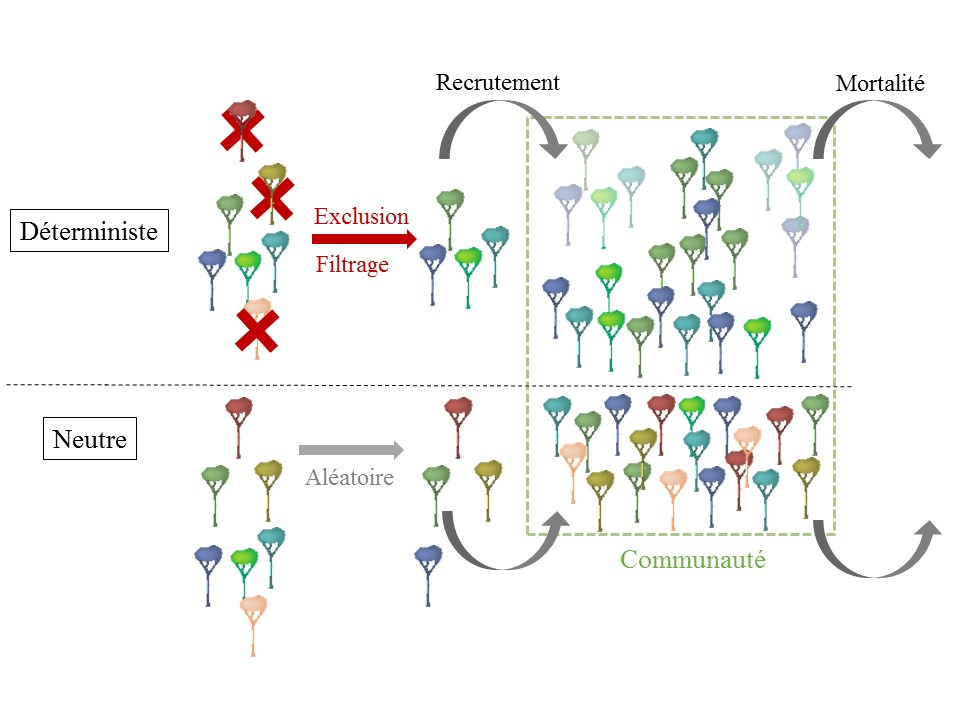
\includegraphics[width=1\linewidth]{ExternalFig/Fig_AssemblyRules} 

}

\caption{Schéma des processus déterminant la réponse des communautés végétales aux perturbations. Les processus déterministes (partie haute) sélectionnent les espèces recrutées dans la communauté selon leurs préférences environnementales e leur compétitivité, tandis que les processus stochastiques (partie basse) reviennent à une sélection aléatoire.}\label{fig:AssemblyRules}
\end{figure*}

\section{Comment mesurer la diversité biologique
?}\label{comment-mesurer-la-diversite-biologique}

Les processus démographiques et les règles d'assemblage d'espèces
déterminent la structure, la composition et la diversité des
communautés. Prédire et gérer l'avenir des forêts et en particularité de
leur précieuse diversité biologique nécessite de comprendre le rôle des
ces différents processus dans la définission de la diversité biologique
dans tous ses aspects. La biodiversité est définie de l'échelle du gène
à celle de l'écosystème considère la diversité des plantes, animaux,
champignons et microorganismes qui constituent les écosystèmes, de leur
variabilité génétique et phénotypique, et de la variabilité de leurs
assemblages \autocite{Loreau2005}. La biodiversité est souvent réduite à
celle de richesse en espèces, mais tient compte en réalité des multiples
aspects de richesse, d'homogenéité, de disparité et d'interactions entre
les éléments du vivant qui constituent les communautés. Appréhender les
différents aspects de la biodiversité permet d'identifier les mécanismes
écologiques fondamentaux qui régissent les écosystèmes et leurs
dynamiques spatiales et temporelles \autocites{Purvis2000}{Loreau2005}.

\subsection{Composition et dissimilarité entre
communautés}\label{composition-et-dissimilarite-entre-communautes}

De nombreuses mesures permettent d'estimer ce turnover, qui prennent en
compte ou non l'abondance des espèces \autocite{Podani2013}. Nous avons
choisis ici de mesurer le taux de remplacement d'abondance, ou
similarité de Bray-Curtis, qui représente dans quelle mesure une
communauté est le sous-ensemble d'une plus grande. En pratique, si la
communauté recrutée après exploitation répond aux mêmes lois que la
communauté initiale elle sera équivalente à une communauté qui en aurait
été tirée au hasard. La similarité de Bray-Curtis mesure la somme des
abondances d'une commaunté remplacées par une espèce différente,
normalisée par l'abondance totale partagée entre les deux communautés
\eqref{eq:formNestedness}.

\begin{equation}
T_{ab}=\frac{\sum_{i=1}^{n}|x_i^a - x_i^b| - \bigg| \sum_{i=1}^{n}{x_i^a} - \sum_{i=1}^{n}{x_i^b} \bigg|}{\sum_{i=1}^{n}\max{\left( x_i^a;x_i^b \right)}}
\label{eq:formNestedness}
\end{equation}

\subsection{Assemblage et structure des
communautés}\label{AbundanceDistribution}

Une communauté, qu'elle soit végétale, animale ou microbienne, est
constituée d'espèces aux effectifs différents: certaines sont très
abondantes, d'autres moyennement communes et d'autres encore, souvent la
majorité, sont rares. La façon la plus simple et immédiate de décrire
une communauté est de donner la distribution d'abondance de ses espèces,
qui représente les proportions d'espèces abondantes rapport aux espèces
communes ou rares. Cette distribution bien que variable d'une communauté
à l'autre, est régie par des lois écologiques lui donnant invariablement
une courbe en creux \ref{fig:AbdDist} \autocite{McGill2007}.

\begin{Shaded}
\begin{Highlighting}[]
\NormalTok{knitr}\OperatorTok{::}\KeywordTok{include_graphics}\NormalTok{(}\StringTok{"ExternalFig/SpeciesAbdDist.jpg"}\NormalTok{)}
\end{Highlighting}
\end{Shaded}

\begin{figure*}

{\centering 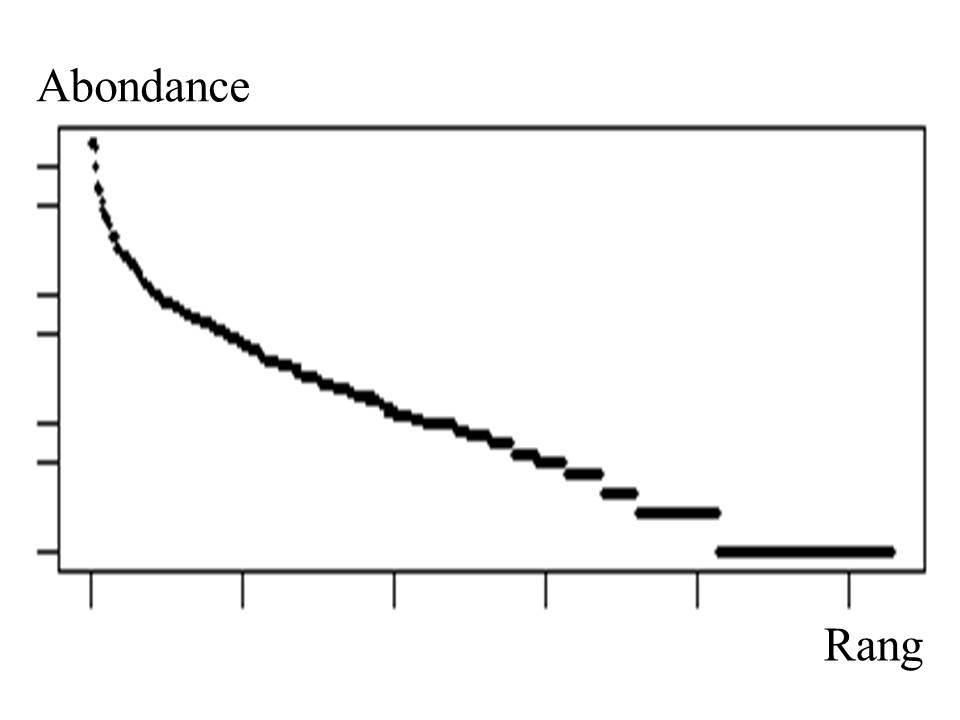
\includegraphics[width=0.6\linewidth]{ExternalFig/SpeciesAbdDist} 

}

\caption{Exemple de distribution d'abondance pour une communauté d'arbres en forêt tropicale humide}\label{fig:AbdDist}
\end{figure*}

Cette uniformité des distributions d'abondance a motivé le développement
de modèles proposant des relations mathématiques entre le nombre
d'espèces et leur abondance. Ces modèles reflètent le lien entre
l'importance d'une espèce dans la communauté et la quantité de
ressources qu'elle mobilise pour son développement: plus une espèce est
compétitive, plus elle sera abondante. Ce lien s'établit vis à vis de la
ressource limitante, qui peut être la lumière, l'eau disponible, les
nutriments du sol, l'espace, etc
\autocites{Silvertown2004}{terSteege2006}. Prédire une distribution
d'abondance revient à prédire la répartition de la ressource limitante
entre les espèces de la communauté. De nombreux modèles prédictifs ont
été proposés, des modèles statistiques divisant aléatoirement la
ressource selon une loi de propabilité donnant les effectifs de chaque
espèce, aux modèles mécanistes divisant la resource selon une formule
prédéterminée, par exemple en la divisant successivement selon une
fraction constante
\autocites{Fisher1943}{Motomura1932}{Tokeshi1993}{Magurran1988}.

Ces modèles testés pour de nombreuses communautés, ont démontré pouvoir
représenter correctement les communautés réelles et révéler les règles
écologiques qui en régissent l'assemblage. Ce sont des outils adéquats
pour comparer les communautés et en interpréter les différences, mais
manipuler une distribution d'abondance reste compliqué car il s'agit
d'une repréentation en 2D et ne permet pas de quantifier les différences
entre communautés. En revanche, les paramètres de ces distributions et
des modèle proposés pour les représenter permettent de quantifier le
nombre d'espèces, la forme des distribution, ou encore l'homogénéité des
abondances. Ces indicateurs sont les indices de diversité, résumant de
façon quantifiable les caractéristiques des distributions d'abondance.

\subsection{Les composantes de la
diversité}\label{les-composantes-de-la-diversite}

Si la biodiversité d'une communauté est souvent assimilée à sa richesse
en espèces, elle englobe en réalité le nombre, l'abondance, la
composition et les interactions entre les espèces. L'abondance en
particulier est essentielle: une espèce dominante n'apportera pas la
même contribution à l'écosystème qu'une espèce rare. Ainsi une
communauté dominée par une ou deux espèces très abondantes sera
intuitivement moins diverse qu'une autre avec autant d'espèces mais aux
abondances équivalentes. L'homogeneité des abondances dans une
population, ou \emph{équitabilité}, peut être bien plus révélatrice du
fonctionnement des écosystèmes que leur richesse ou leur composition.
Cette idée est illustrée par l'hypothèse du ratio de biomasse selon
laquelle les espèces dominantes sont bien plus déterminantes du
fonctionnement des écosystèmes que les espèces rares. Les espèces peu
communes n'ont une influence qu'à long terme, en tant que potentielles
futures espèces dominantes si l'environnement change, ou pas d'influence
si elles sont transitoires et ne persistent pas dans l'écosystème
\autocite{Grime1998}.

La richesse, simplement le nombre d'espèces recensées, et
l'équitabilité, la régularité de distribution d'abondance des espèces,
sont donc les deux composantes de la diversité taxonomique d'une
communauté \ref{fig:RichEqu} \autocites{Whittaker1965}{Magurran2004}.

\begin{Shaded}
\begin{Highlighting}[]
\NormalTok{knitr}\OperatorTok{::}\KeywordTok{include_graphics}\NormalTok{(}\StringTok{"ExternalFig/Fig_RichnessEquitability.jpg"}\NormalTok{)}
\end{Highlighting}
\end{Shaded}

\begin{figure*}

{\centering 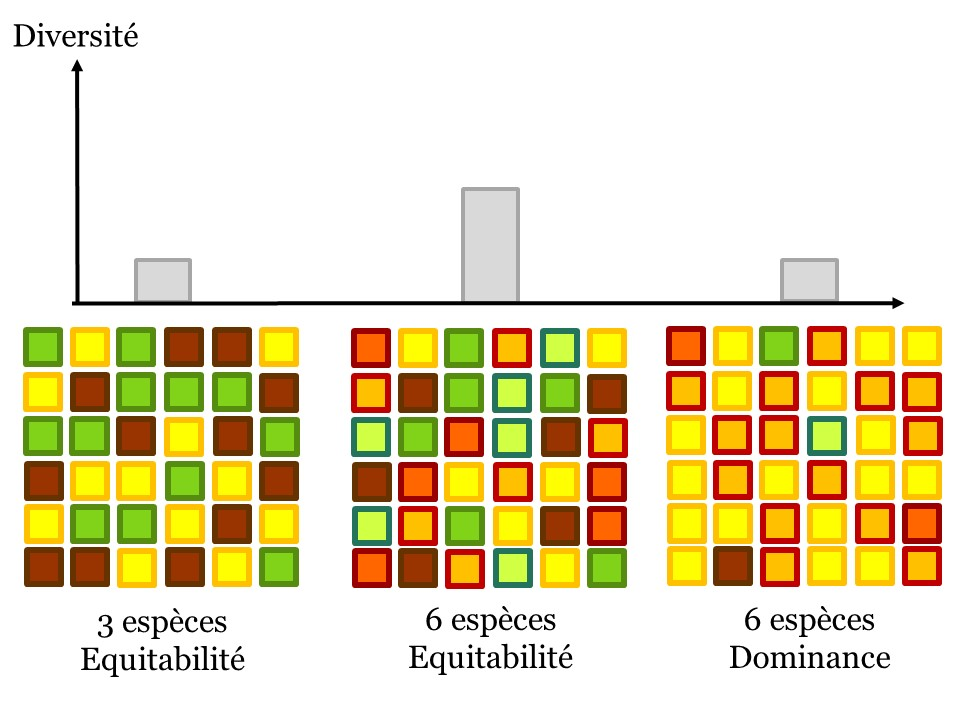
\includegraphics[width=0.6\linewidth]{ExternalFig/Fig_RichnessEquitability} 

}

\caption{Les deux composantes de la diversité taxonomique: richesse (nombre d'espèces) et équitabilité (homogeneité de répartition)}\label{fig:RichEqu}
\end{figure*}

Mesurer la diversité ne revient donc pas à une mesure unique mais
plusieurs indices de diversité qui combinent différemment les
composantes de la diversité. Plusieurs familles d'indices de diversité
ont été développées et regroupent les indices mesurés selon une même
formule dont les déclinaisons accordent un poids variables aux
composantes de la diversité. La famille des indices de diversité de
Réyni par exemple, judicieuse pour l'étude des communautés végétales,
rassemble les indices mesurés selon l'équation \eqref{eq:formHCDT} modulée
par un paramètre \emph{q} appelé ``ordre de diversité'' qui correspond
au poids des espèces rares par rapport aux espèces abondantes
\autocite{Mendes2008}. Plus l'ordre de diversité est élevé, plus les
espèces rares sont négligées par rapport aux espèces abondantes.

\begin{equation}
{^{q}H=\frac{1}{q-1}\Bigg(1-\displaystyle\sum_{s=1}^{S}p^q_s\Bigg) }
\label{eq:formHCDT}
\end{equation}

Dans cette famille d'indices de diversité se retrouvent les indices les
plus utilisés dans la littérature: l'ordre 0 où chaque espèce contribue
de la même façon correspond à la richesse spécifique, l'ordre 1 où
richesse et équitabilité sont également prises en compte correspond à
l'indice de Shannon, et l'ordre 2 pour lequel les espèces rares sont
presque négligées correspond à l'indice de Simpson (parfois appelé
``diversité en espèces abondantes'')
\autocites{Shannon1948}{Simpson1949}{Patil1982}{Tothmeresz1995}.

Ces indices, mathématiquement corrects et représentatifs des différentes
composantes de la diversité, ne donnent cependant pas un nombre
intelligible qui permettent de comparer facilement différentes
communautés. Les indices de diversité doivent être traduits en
\emph{nombre équivalent d'espèces} qui correspond au nombre d'espèces
qu'aurait la communauté étudiée si toutes les espèces avaient la même
abondance. Ce nombre équivalent d'espèces, ou \emph{nombre de Hill}, est
obtenu par transformation des valeurs obtenues par une exponentielle à
base q \autocite{Hill1973}.

Les mesures de diversité choisies sont donc la traduction intelligible
en nombre équivalent d'espèces d'une déclinaison d'indices combinant
richesse et équitabilité de différentes façons pour capter toute
structure de diversité.

\subsection{Résolution du biais
d'échantillonnage}\label{resolution-du-biais-dechantillonnage}

En pratique aucun inventaire n'est exhaustif et l'étude de la diversité
se heurte aux biais d'échantillonnage qui sous-estiment la richesse et
faussent l'abondance des espèces. Corriger ce biais nécessite d'estimer
les abondances réelles à partir des observations et des relations
mathématiques reliant les abondances des différentes espèces. La
première méthode développée correspond à la formule des fréquences de
Turing \autocite{Good1953} où l'abondance réelle *\alpha\_v* d'une
espèce observée \emph{v} fois dans un échantillonnage de \emph{n}
individus dépend du nombre d'espèces observées également \emph{v} fois
et d'e celles'espèces observées \emph{v+1} fois
@ref\{eq=formGoodTuring\}:

\begin{equation}
\alpha_v=\frac{\big(v+1\big)}{n}\frac{s^n_{v+1}}{s^n_v}
\label{eq:formGoodTuring}
\end{equation}

Les singletons (espèces observées une seule fois) et les doubletons
(espèces observées deux fois) sont alors particulièrement intéressants
car il permettent d'estimer le nombre \emph{s\^{}n\_0} d'espèces
observées zéro fois (\(s^n_0=\frac{s^n_1}{n}\)) qui ont été manquées
dans l'inventaire et peuvent être ajoutées aux observation pour corriger
le biais d'échantillonnage de la richesse.

De nombreuses méthodes ont repris cette relation en y intégrant
notamment la notion de \emph{taux de couverture} qui quantifie l'effort
d'échantillonnage d'un inventaire réel et permet de savoir quelle
proportion de la communauté est échantillonnée \autocite{Dauby2012}. La
correction la plus adéquate a pu être déterminée selon le taux de
couverture de l'inventaire et les estimateurs de la diversité sont
aujourd'hui très fiables \autocites{Chao2015}{Marcon2015b}.

\subsection{Diversité fonctionnelle}\label{diversite-fonctionnelle}

Les mesures de diversité décrites précédemment, appelées diversité
neutre, considèrent toutes les espèces de la même façon que celles-ci
aient ou non des caractéristiques biologiques ou phylogénétiques
proches. Ces diversités peuvent cependant facilement intégrer les
caractéristiques des espèces en mesurant leur similarité et une
communauté sera d'autant plus diverse que les espèces qui la constituent
sont différentes. Pour des communautés végétales la diversité
phylogénétique considère les distances entre espèces dans un arbre
phylogénétique et la diversité fonctionnelle considère leurs différences
morphologiques ou physiologiques \ref{fig:RichEquSim}.

\begin{Shaded}
\begin{Highlighting}[]
\NormalTok{knitr}\OperatorTok{::}\KeywordTok{include_graphics}\NormalTok{(}\StringTok{"ExternalFig/Fig_RichnessEquitabilitySimilarity.jpg"}\NormalTok{)}
\end{Highlighting}
\end{Shaded}

\begin{figure*}

{\centering 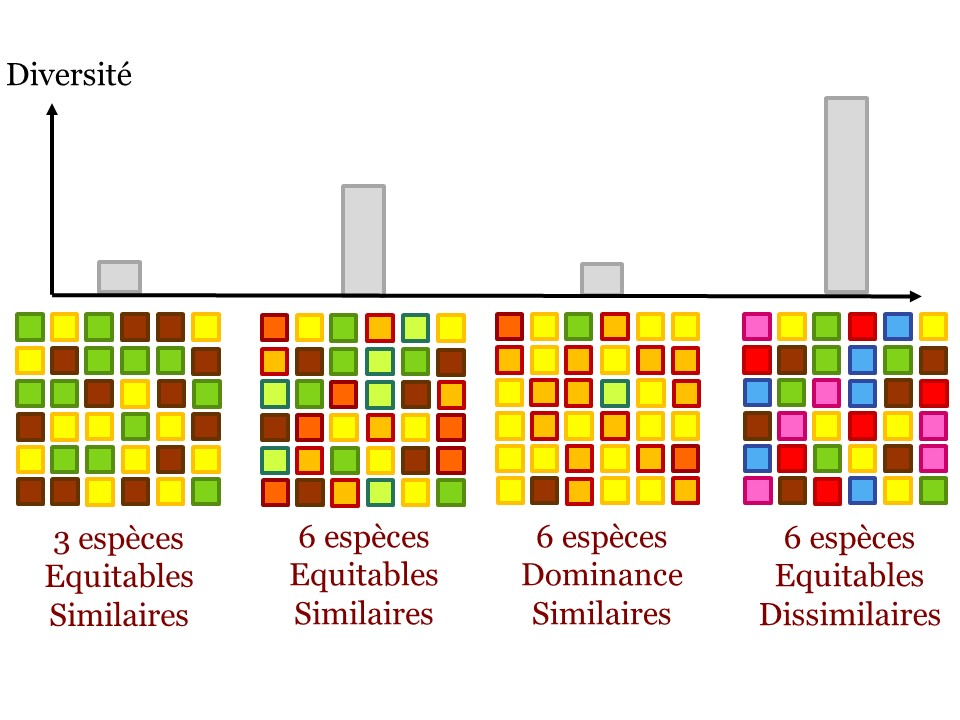
\includegraphics[width=0.6\linewidth]{ExternalFig/Fig_RichnessEquitabilitySimilarity} 

}

\caption{Troisième composante de la diversité: la similarité entre espèces basée sur des distances phylogénétiques ou taxonomiques}\label{fig:RichEquSim}
\end{figure*}

Ces similarités sont ensuite intégrées aux indices de diversité, au même
titre que la richesse et l'équitabilité, sous la forme d'une matrice de
distances entre espèces calculée sur la base de leur phylogénie ou de
leurs traits fonctionnels.

Les traits fonctionnels sont les caractéristiques morphologiques,
physiologiques et phénologiques des espèces, ils déterminent le
fonctionnement des individus, leur performance de croissance et de
survie, et leurs interaction avec l'environnement
\autocite{Violle2007b}. L'approche fonctionnelle décrivant les espèces
et les individus selon leurs caractéristiques biologiques a été
largement adoptée en écologie. D'une part, cette approche réduit la
dimensionnalité des communautés, indispensable pour l'étude
d'écosystèmes aussi riches que les forêts tropicales et permet de
comparer les communautés quelle que soit leur composition en espèces
\autocites{Begon2006}{Scheiter2013}{Mouillot2013a}{Sakschewski2016}.
D'autre part, composition et diversité fonctionnelle sont interprétables
en termes d'utilisation des ressources et de flux de matière et
d'énergie, et relient directement la diversité des communautés à leur
fonctionnement. Enfin, cette approche appréhende la signature
fonctionnelle des perturbations et permet d'identifier et de quantifier
les processus déterminant la dynamique des communautés
\autocite{Funk2017}. La définition des processus déterministes est
qu'ils n'impliquent pas les espèces de la même façon selon leurs
caractéristiques biologiques: l'exclusion abiotique d'espèces non
adaptées à l'environnement se traduiront par une aggrégation de la
communauté dans l'espace des traits fonctionnels et une diminution de sa
diversité fonctionnelle, tandis que l'exclusion compétitive limitant les
similarité entre espèces se traduira par une dispersion des traits
fonctionnels de la communauté et une diversité fonctionnelle élevée
\autocites{McGill2006}{Kunstler2012}.

L'approche fonctionnelle nécessite de choisir judicieusement les traits
intégrés aux indices de diversité. Une vaste littérature a permis
d'identifier les traits clés représentatifs de l'écologie et de la
croissance des espèces et de leur influence sur le fonctionnement de
l'écosystème \autocite{Reich2014}. Les traits foliaires tout d'abord,
qui déterminent la stratégie d'acquisition et d'allocation des resources
lumineuses, définissent un ``spectre économique foliaire'' qui oppose
les espèces à larges feuilles fines ayant une forte capacité
photosynthétique permettant une acquisition rapide des resources, aux
espèces à petites feuilles coriaces et résistantes. Un gradient
similaire s'applique aux traits racinaires et aux propriétés du bois,
opposant les espèces aux tissus légers à courte durée de vie permettant
une croissance rapide à celles aux tissus denses plus résistants et
mobilisant plus de ressources
\autocites{Chave2009}{Valverde-Barrantes2017}. Les stratégies
d'acquisition des resources déterminent la stratégie de croissance des
espèces: les espèces ``acquisitives'' auront une croissance rapide et
une courte durée de vie tandis que les espèces ``conservatives'' auront
une croissance plus lente mais une meilleure résistance aux conditions
environnementales éprouvantes \autocites{Reich1997}{Wright2004}. A ces
traits fonctionnels mesurables à l'échelle de l'individus s'ajoutent des
\emph{traits d'histoire de vie} mesurables à l'échelle de l'espèce.
Parmi ces traits la masse des graines et la hauteur moyenne maximale des
arbres à l'âge adulte ont montré être particulièrement représentatifs
des stratégies de croissance, de survie et de reproduction
\autocites{Westoby1998}{Herault2011}. La combinaison de l'ensemble de
ces traits spécifique, foliaires, racinaires et du bois appréhende la
stratégie fonctionnelle des espèces, leurs préférences écologiques et
leur performance de croissance et de survie. L'engouement récent de
l'écologie pour l'approche fonctionnelle a de plus permis la création de
bases de données fonctionnelles conséquentes et standardisées qui
rendent possibles l'approche fonctionnelle à l'échelle des communautés
{[}\textcite{Kattge2011}; \textcite{Perez-Harguindeguy2013}; \footnote{\url{http://www.ecofog.gf/Bridge/}}{]}

L'approche fonctionnelle considère la diversité des communautés mais
également leur composition fonctionnelle mesurable par les valeurs
moyennes de traits pondérées par l'abondance des espèces
(\emph{Community Weighted Means, CWM} en anglais). L'abondance des
caractéristiques fonctionnelles détermine à la fois le fonctionnement
des communautés et leur résilience. D'après la théorie du ``ratio de
biomasse'' \autocite{Grime1998}, le rôle d'un individu dans l'écosystème
dépend de la fraction de biomasse qu'il représente et le fonctionnement
des communautés repose sur les espèces dominantes tandis que les espèces
rares ont peu d'influence. Par ailleurs la répartition d'abondance des
traits fonctionnels amène à la notion de redondance fonctionnelle qui
quantifie le nombre d'espèces partageant les mêmes valeurs de traits. La
redondance fonctionnelle, souvent élevée en forêt tropicale, permet aux
communautés de perdre des espèces sans nécessairement voir disparaître
leur rôle dans l'écosystème: la redondance détermine en partie la
résilience des communautés et atténue l'impact des perturbations.
L'organisation de la redondance dans l'espace des traits d'une
communauté renseigne sur les assemblages les plus stables qui se
dégageraient le plus probablement après de nouvelles perturbations. La
redondance fonctionnelle d'une communauté peut se mesurer dans l'espace
fonctionnel à partir de la densité de probabilité de traits
(\emph{Traits Density Probability, TDP} en anglais) de chaque espèce
\autocite{Carmona2016}. Les densités des espèces d'une communauté
pondérées par leur abondance sont additionnées pour donner la redondance
fonctionnelle sur l'ensemble de l'espace fonctionnel ou sur un espace
restreint, comme nous le ferons par la suite quand on s'intéressera à la
redondance fonctionnelle dans l'espace de la communauté de départ
\ref{fig:RedundancyMethod}.

\begin{Shaded}
\begin{Highlighting}[]
\NormalTok{knitr}\OperatorTok{::}\KeywordTok{include_graphics}\NormalTok{(}\StringTok{"ExternalFig/Fig_MesureRedondance.jpg"}\NormalTok{)}
\end{Highlighting}
\end{Shaded}

\begin{figure*}

{\centering 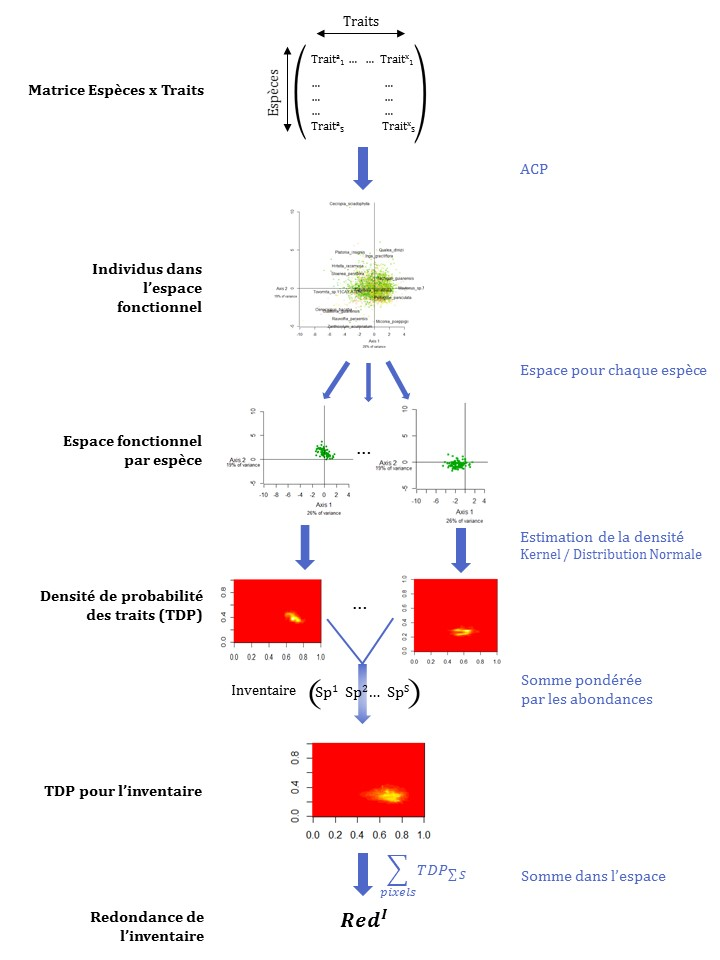
\includegraphics[width=0.8\linewidth]{ExternalFig/Fig_MesureRedondance} 

}

\caption{La redondance fonctionnelle est la somme des chevauchement entre espèces dans l'espace fonctionnel. Les individus de la base de données fonctionnelle sont représentés dans un espace à 2 dimensions grâce à une analyse en composantes principales (ACP). Une estimation par noyau estime ensuite la densité de probabilité des traits (TDP) de chaque espèce. La somme de ces densités pondérées par l'abondance des espèces donne enfin la redondance fonctionnelle de la communauté, interprétable comme le nombre d'espèces qui peuvent disparaître sans diminuer l'espace fonctionnel de la communauté.}\label{fig:RedundancyMethod}
\end{figure*}

\section{La Guyane Française et l'exemple de la station de
Paracou}\label{la-guyane-francaise-et-lexemple-de-la-station-de-paracou}

Le bassin Amazonien est la plus riche des trois principales régions de
forêt tropicale humide \autocite{Gentry1988} et la Guyane française en
est une région de 83 846 km\^{}2 recouverte à 95\% forestière au
Nord-Est du continent sud-américain entre le Surinam et le Brésil.

\subsection{Le contexte Guyanais}\label{le-contexte-guyanais}

La région appartient au bouclier des Guyanes qui s'étend de l'Amapa au
Brésil jusqu'au delta de l'Orénoque au Venezuela. Formé il y a plus de 2
milliards d'années, le bouclier des Guyanes est un assemblage d'unités
géomorphologiques façonnées par une succession d'épisodes géologiques,
climatiques et marins. Ces unités correspondent à des conditions
pédologiques, climatiques et topographiques déterminant la composition
et la diversité du couvert végétal et les processus écologiques qui les
régissent, tels que les migrations et le filtrage environnemental
\autocite{Guitet2015}.

Le relief Guyanais est une grande diversité topographique qui alterne
entre des collines allant jusqu'à 50m d'altitude, et des bas-fonds
humides. Les sols sont des Acrisols recouvrant une couche de saprolite
transformée peu perméable qui entraîne un drainage latéral des
précipitations. La profondeur des sols, leur composition et leur
capacité de rétention et de drainage de l'eau sont très hétérogènes
\autocites{Ferry2010}{Robert2003}.

Le climat est un climat tropical humide, davantage marqué par le régime
des précipitations que par celui des températures. La température
moyenne est 26°C et reste constante au cours de l'année tandis les
précipitations moyennes annuelles varient de 2 000 à 4 000
mm.an\textsuperscript{-1} et montrent une grande variabilité spatiale et
temporelle. Les précitations suivent un gradient décroissant marqué
d'est en ouest et une forte variabilité au cours de l'année, avec une
saison humide entre novembre et avril et une saison sèche d'avril à
mi-juillet durant laquelle les précipitations sont inférieures à 50 mm
\autocite{Wagner2011}.

La forêt Guyanaise est une forêt équatoriale sempervirente ombrophile de
plaine. D'une richesse incroyable, elle accueille plus de 7 000 espèces
végétales (hors champignons) dont 1 500 espèces d'arbres et une richesse
faunistique toute aussi incroyable \autocite{DeNoter2008}. La
composition taxonomique des arbres est très variable sur le territoire.
Plusieurs patrons de composition on été mis en évidence selon un
gradient du nord-ouest où dominent les familles botaniques des
\emph{Lecythidaceae} et \emph{Cesalpinaceae}, au sud-est où dominent
\emph{Burseraceae} et \emph{Mimosaceae}. Ces patrons suivent en
particulier par une combinaison de gradients topographique et
pédologique \autocites{Sabatier1989}[ cf
Toto]{Sabatier1997}{Guitet2015}.

\subsection{Paracou, plus de 30 de suivi de la forêt
Amazonienne}\label{paracou-plus-de-30-de-suivi-de-la-foret-amazonienne}

Le dispositif de Paracou, installé entre les communes de Kourou et
Sinnamary (5°18'N and 52°53'W), a été mis en place en 1984 pour étudier
l'impact de l'exploitation forestière sélective sur les peuplements
forestiers. Le dispositif correspond à l'origine à 12 parcelles de 6.25
ha ayant subi en 1984 un gradient de trois intensités d'abattage,
d'éclairices et de coupe de bois de chauffage. Le traitement de
perturbation a été attribué selon un dispositif aléatoire de trois
réplications de 4 traitements: parcelles témoins sans intervention
(\emph{T0}), traitement 1 avec coupes d'abattage (\emph{T1}), traitement
2 avec abattage et éclaircies par \textbf{poison girdling} (\emph{T2}),
traitement 3 avec abattage, éclaircies et coupe de bois de chauffage
(\emph{T3}) \ref{tab:InterventionTable}.

En 1990, trois parcelles de 6.25ha et une parcelle de 25ha (parcelles
13, 14, 15 et 16) ont été ajoutées au dispositif pour l'étude et le
suivi de la diversité en forêt non perturbée \ref{fig:ParacouDesign}.

\begin{Shaded}
\begin{Highlighting}[]
\NormalTok{knitr}\OperatorTok{::}\KeywordTok{include_graphics}\NormalTok{(}\StringTok{"ExternalFig/Paracou.jpg"}\NormalTok{)}
\end{Highlighting}
\end{Shaded}

\begin{figure*}

{\centering \includegraphics[width=0.6\linewidth]{ExternalFig/Paracou} 

}

\caption{Dispositif expérimental de Paracou, schéma des 16 parcelles de suivi des dynamiques forestières. La couleur des parcelles indique l'intensité de perturbation appliquée à 9 des parcelles en 1984 (voir le tableau 1.}\label{fig:ParacouDesign}
\end{figure*}

Sur l'ensemble du dispositif sont recensées 591 espèces d'arbres
appartenant à 223 genre et 64 familles botaniques, principalement les
\emph{Fabaceae}, les \emph{Chrisobalanaceae}, les \emph{Lecythidaceae}
et les \emph{Sapotaceae}. Les températures annuelles atteignent 26°C et
les précipitations 2 980 mm.an\textsuperscript{-1} de mi-août à
mi-novembre, avec une saison sèche d'un mois en mars
\autocite{Wagner2011}.

\subsection{Méthodes d'inventaires}\label{methodes-dinventaires}

Depuis la mise en place du dispositif en 1984 toutes les parcelles sont
inventoriées chaque année à la saison sèche à partir de mi-juillet. Tous
les arbres de plus de 10 cm de diamètre à 1.30 m (diamètre à hauteur de
poitrine, \emph{DBH} en anglais) sont identifiés, numérotés et
cartographiés. Les arbres morts sont relevés chaque année et notés en
précisant le type mort (mort sur pied, chablis primaire ou chablis
secondaire).

Lorsqu'un arbre atteint 10 cm il est \emph{recruté} et sera mesuré
chaque année. Il est identifié dans un premier temps par un nom
\emph{vernaculaire}, ou nom commun, attribué par l'équipe de terrain. En
1984, 62 espèces commerciales étaient identifiées par un nom commun
propre tandis que toutes les autres espèces étaient regroupées sous deux
noms vernaculaires distinguant les palmiers des espèces arborées. Cette
identification en nom vernaculaire s'est précisée par la suite et
aujourd'hui 235 noms vernaculaires différents sont recensés pour
l'ensemble du dispositif sur les 30 ans de suivi. Des campagnes
d'identification botanique au cours desquelles les arbres sont
identifiés au niveau espèce botanique ont été mises en place à partir de
2003 et se poursuivent depuis tous les 5 à 6 ans.

L'histoire des inventaires botaniques s'étant construite petit à petit
au gré des nouveaux projets et des forces en présence, la précision et
le taux d'identification botaniques sont variables au cours du temps et
entre les parcelles. Ceci génère des incertitudes taxonomiques
importantes, les noms vernaculaires correspondant souvent à plusieurs
noms botaniques et inversement \autocite{Oldeman1968}. Le soucis vient
alors des arbres n'ayant qu'un identification en nom vernaculair,
lorsque l'individu est mort avant d'avoir pu être identifié au cours
d'une campagne botanique par exemple.

\section{Problématique et plan de la
thèse}\label{problematique-et-plan-de-la-these}

La thèse présentée ici cherche à déterminer la réponse aux perturbations
d'une forêt tropicale naturelle en termes de diversité taxonomique et
fonctionnelle, à en interpréter les mécanismes sous-jacents et à
clarifier la résilience des forêts tropicales dans le contexte des
changements actuel. Le document s'organise en trois chapitres
correspondant à trois articles scientifiques en cours de rédaction (pour
le moment!).

\begin{itemize}
\tightlist
\item
  Le premier chapitre présente une méthode de propagation des
  incertitudes taxonomiques permettant d'estimer la diversité en tenant
  compte des indéterminations botaniques. La méthode se base sur des
  inventaires théoriques complets reconstitués à partir des associations
  entre noms vernaculaires et botaniques. Ces associations peuvent être
  estimées à partir d'inventaires réels ou à partir de dires d'experts,
  correspondant à l'interview des équipes d'ouvriers forestiers
  réalisant les inventaires: les permiers développement permettent de
  tester la robustesse de la méthode en fonction de l'information
  considérée et de la calibrer de façon optimale.
\end{itemize}

Nous proposons ensuite l'application de cette méthode à des inventaires
forestiers réels. Ces inventaires, réalisés à large échelle dans le
cadre de l'exploitation forestière permettraient d'élargir l'étude de la
biodiversité forestière dans le temps et l'espace mais restent peu
précis. La méthode développée ici permet d'améliorer la précision
botanique et de proposer une méthode dinventaire optimisée pour valorise
rau mieux ces inventaires.

Nous proposons ensuite l'application de cette méthode aux dispositifs
expérimentaux, dont les contraintes d'identification sont différentes,
et qui sera utilisée dans la suite de ce travail.

\begin{itemize}
\item
  Dans le deuxième chapitre nous allons étudier les trajectoires de
  composition et de diversité taxonomique et fonctionnelle des parcelles
  de Paracou. Nous verrons quelles sont les conséquences à long terme
  des perturbations sur le fonctionnement des communautés et pourrons
  identifier les processus écologiques régissant cette dynamique. En
  particulier nous testons la validité de la théorie des perturbations
  intermédiaires, qui prédit une diversité maximale lorsque des
  perturbations moyennes permettent un renouveau des espèces présentes
  mais ne permettent pas l'hyperdominance d'un nombre restreint
  d'espèces. Les trajectoires permettent de plus de discuter des
  différents aspect de la résilience des communautés et de développer
  des hypothèses concernant l'avenir des forêts.
\item
  Le troisième chapitre met l'accent sur les processus de recrutement et
  leur rôle pour la résilience des forêts tropicales. S'intéresser au
  recrutment revient à décrire la forêt mise en place à plus ou moins
  long terme après perturbation ainsi que les processus écologiques
  sous-jacents. Les trajectoires de recrutement on permet d'identifier
  la succession des phases de recrutement après exploitation et d'en
  décrire les différents processus écologiques de sélection qui
  régissent l'assemblage de la future forêt. Ces conclusions ont permis
  de discuter la résilience des processus eux-mêmes et d'anticiper la
  réponse à de nouvelles perturbations.
\end{itemize}

\chapter{Article 1 : Des inventaires forestiers aux trajectoires de
diversité: le problème universel de
l'incertitude}\label{article-1-des-inventaires-forestiers-aux-trajectoires-de-diversite-le-probleme-universel-de-lincertitude}

Malgré les enjeux liés aux forêts tropicales et l'urgence d'en préserver
l'intégrité et le fonctionnement, seule une petite fraction de leur
diversité est connue. Le nombre d'espèces inventoriées sous les
tropiques ne correspondant qu'à une observation unique
\autocite{Feeley2011} présume de l'ampleur de notre méconnaissance et
rend impossible toute supposition sur la distribution des espèces et
leurs dynamiques. Il est essentiel d'améliorer notre connaissance du
vivant, en fournissant un plus grand effort d'échantillonnage et en
valorisant toute connaissance déjà disponible.

Le coût des inventaires en temps, en main d'oeuvre et en moyens,
d'autant plus important que le niveau de l'inventaire est précis,
implique de travailler également à des méthodes pour valoriser tout type
d'inventaires \autocite{Baraloto2012}. Dans le cas de l'étude des
peuplements forestiers, les inventaires d'exploitation peu coûteux et
couvrant des surfaces larges sont une source d'information
incontournable \autocites{terSteege2000}{Guitet2014}.

\section{Noms vernaculaires et propagation des incertitudes
taxonomiques}\label{noms-vernaculaires-et-propagation-des-incertitudes-taxonomiques}

Ces inventaires ne sont cependant généralement pas réalisés en noms
scientifiques mais noms vernaculaires, qui sont mieux connus, plus
faciles à attribués car basés sur des critères morphologiques, culturels
ou d'usage et qui ne nécessitent pas de vérification botanique
ultérieure à partir d'herbiers. Cette simplicité se fait cependant au
détriment de la fiabilité des noms vernaculaires, qui correspondent à
plusieurs espèces botaniques et varient avec le temps et les équipes de
terrain \autocite{Oldeman1968}. Pour valoriser ces inventaires il est
donc nécessaire d'évaluer l'impact de l'incertitude taxonomique sur la
fiabilité et la sensibilité des mesures de diversité. Nous proposons ici
une méthode permettant de propager l'incertitude de détermination
taxonomique des noms vernaculaires aux mesures de la diversité.

Dans un premier temps nous appliquons cette méthode au contexte des
inventaires d'exploitation en noms vernaculaires pour en estimer la
fiabilité et la robustesse selon le degré d'indétermination botanique,
et proposer un protocole d'inventaire standardisé. Dans ce cas les
identifications botaniques fiables concernent quelques espèces cibles,
emblématiques ou ayant une certaine valeur commerciale ou de
conservation. Le degré d'indétermination botanique correspond alors au
nombre d'espèces identifiées systématiquement par leur nom vernaculaire
plutôt que botanique. Dans un deuxième temps nous adaptons la méthode au
contexte des dispositifs expérimentaux pour pallier l'inévitable
variabilité des pratiques d'inventaires. Dans ce cas les arbres
identifiés uniquement par un nom vernaculaire sont les individus n'ayant
pu être identifiés, que l'identification soit impossible ou qu'ils
soient mort avant le passage du taxonomiste. Le degré d'indétermination
correspond au nombre d'arbres sans identification botanique et concerne
potentiellement toutes les espèces de la communauté.

\section{Article 1 \_ Inescapable Taxonomists: Workable Biodiversity
Management Must Base on a Minimum Field
Work}\label{article-1-_-inescapable-taxonomists-workable-biodiversity-management-must-base-on-a-minimum-field-work}

\section{La recherche et les suivis à long terme: application de la
méthode de propagation aux inventaires de
Paracou}\label{la-recherche-et-les-suivis-a-long-terme-application-de-la-methode-de-propagation-aux-inventaires-de-paracou}

\subsection{Profils d'incertitude
taxonomique}\label{profils-dincertitude-taxonomique}

A la différence des inventaires d'exploitation, dans le cas des
dispositifs expérimentaux le degré d'indétermination taxonomique
correspond à un pourcentage d'arbres, toutes espèces confondues, n'ayant
pas été identifiés au niveau spécifique. Sur le même principe que pour
les inventaires d'exploitation, nous avons simulé un gradient
d'indétermination taxonomique à partir d'inventaires complets en nom
botanique complets évaluer l'impact de l'incertitude taxonomique pour
les mesures de diversité \ref{fig:FigTreesSp}.

\begin{Shaded}
\begin{Highlighting}[]
\KeywordTok{load}\NormalTok{(}\StringTok{"ExternalFig/Uncertaintypropagation_Genus_noCorrection"}\NormalTok{)}

\KeywordTok{par}\NormalTok{(}\DataTypeTok{mfrow =} \KeywordTok{c}\NormalTok{(}\DecValTok{1}\NormalTok{, }\DecValTok{3}\NormalTok{), }\DataTypeTok{no.readonly =} \OtherTok{TRUE}\NormalTok{)}
\KeywordTok{invisible}\NormalTok{(}\KeywordTok{lapply}\NormalTok{(Profile_Genus, }\ControlFlowTok{function}\NormalTok{(ind) \{}
    \KeywordTok{plot}\NormalTok{(}\KeywordTok{colnames}\NormalTok{(ind), ind[}\StringTok{"0.5"}\NormalTok{, ], }\DataTypeTok{type =} \StringTok{"n"}\NormalTok{, }\DataTypeTok{ylim =} \KeywordTok{c}\NormalTok{(}\DecValTok{0}\NormalTok{, }\KeywordTok{max}\NormalTok{(ind)), }\DataTypeTok{xlab =} \StringTok{""}\NormalTok{, }
        \DataTypeTok{ylab =} \StringTok{""}\NormalTok{)}
    \KeywordTok{polygon}\NormalTok{(}\KeywordTok{c}\NormalTok{(}\KeywordTok{colnames}\NormalTok{(ind), }\KeywordTok{rev}\NormalTok{(}\KeywordTok{colnames}\NormalTok{(ind))), }\KeywordTok{c}\NormalTok{(}\KeywordTok{pmax}\NormalTok{(ind[}\StringTok{"0.025"}\NormalTok{, ]), }\KeywordTok{pmin}\NormalTok{(}\KeywordTok{rev}\NormalTok{(ind[}\StringTok{"0.975"}\NormalTok{, }
\NormalTok{        ]))), }\DataTypeTok{col =} \StringTok{"gray75"}\NormalTok{)}
    \KeywordTok{lines}\NormalTok{(}\KeywordTok{colnames}\NormalTok{(ind), ind[}\StringTok{"0.5"}\NormalTok{, ], }\DataTypeTok{col =} \StringTok{"red"}\NormalTok{, }\DataTypeTok{lty =} \DecValTok{2}\NormalTok{)}
    \KeywordTok{points}\NormalTok{(}\KeywordTok{colnames}\NormalTok{(ind), ind[}\StringTok{"0.5"}\NormalTok{, ], }\DataTypeTok{col =} \StringTok{"black"}\NormalTok{, }\DataTypeTok{pch =} \DecValTok{3}\NormalTok{)}
    \KeywordTok{abline}\NormalTok{(}\DataTypeTok{h =}\NormalTok{ ind[}\StringTok{"0.5"}\NormalTok{, }\DecValTok{1}\NormalTok{], }\DataTypeTok{col =} \StringTok{"red"}\NormalTok{, }\DataTypeTok{lty =} \DecValTok{2}\NormalTok{)}
\NormalTok{\}))}
\KeywordTok{mtext}\NormalTok{(}\StringTok{"Incertitude (%)"}\NormalTok{, }\DataTypeTok{side =} \DecValTok{1}\NormalTok{, }\DataTypeTok{cex =} \FloatTok{0.8}\NormalTok{, }\DataTypeTok{outer =} \OtherTok{TRUE}\NormalTok{, }\DataTypeTok{line =} \OperatorTok{-}\DecValTok{2}\NormalTok{, }\DataTypeTok{adj =} \DecValTok{1}\NormalTok{)}
\KeywordTok{mtext}\NormalTok{(}\StringTok{"Diversité équivalente (Espèces)"}\NormalTok{, }\DataTypeTok{side =} \DecValTok{2}\NormalTok{, }\DataTypeTok{padj =} \DecValTok{1}\NormalTok{, }\DataTypeTok{cex =} \FloatTok{0.8}\NormalTok{, }\DataTypeTok{line =} \OperatorTok{-}\FloatTok{0.5}\NormalTok{, }
    \DataTypeTok{outer =} \OtherTok{TRUE}\NormalTok{)}
\KeywordTok{mtext}\NormalTok{(}\StringTok{"Richness"}\NormalTok{, }\DataTypeTok{at =} \FloatTok{0.1}\NormalTok{, }\DataTypeTok{line =} \OperatorTok{-}\FloatTok{1.5}\NormalTok{, }\DataTypeTok{outer =} \OtherTok{TRUE}\NormalTok{)}
\KeywordTok{mtext}\NormalTok{(}\StringTok{"Shannon"}\NormalTok{, }\DataTypeTok{at =} \FloatTok{0.44}\NormalTok{, }\DataTypeTok{line =} \OperatorTok{-}\FloatTok{1.5}\NormalTok{, }\DataTypeTok{outer =} \OtherTok{TRUE}\NormalTok{)}
\KeywordTok{mtext}\NormalTok{(}\StringTok{"Simpson"}\NormalTok{, }\DataTypeTok{at =} \FloatTok{0.76}\NormalTok{, }\DataTypeTok{line =} \OperatorTok{-}\FloatTok{1.5}\NormalTok{, }\DataTypeTok{outer =} \OtherTok{TRUE}\NormalTok{)}
\end{Highlighting}
\end{Shaded}

\begin{figure*}

{\centering 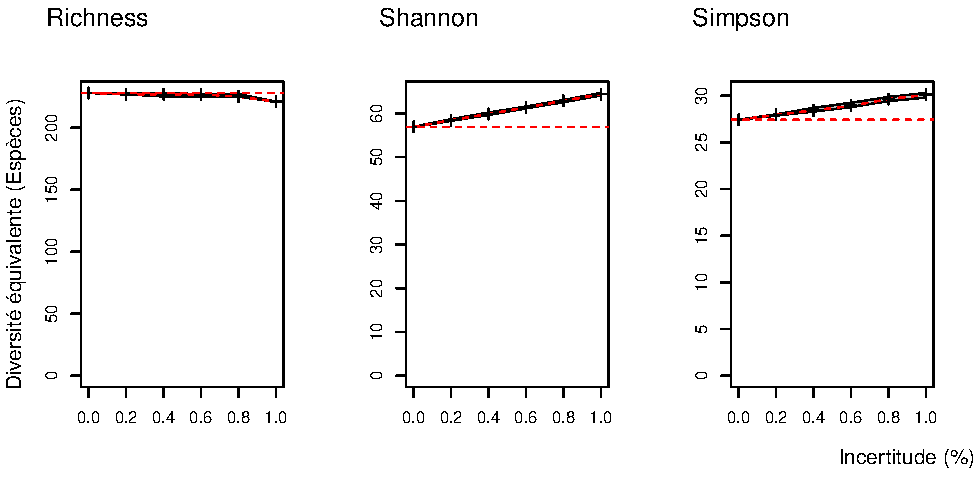
\includegraphics[width=0.6\linewidth]{MyBook_files/figure-latex/FigTreesSp-1} 

}

\caption{Profil de biais pour les diversité de Richesse, Shannon et Simpson au niveau spécifique le long d'un gradient d'indétermination correspondant au pourcentage d'individus identifiés uniquement par leur nom vernaculaire. Les profils de biais représentent la moyenne et les quantiles 0.025 et 0.975 de la distribution des diversités obtenues pour 100 simulations de tirage aléatoire et de propagation des incertitudes.}\label{fig:FigTreesSp}
\end{figure*}

Le profil de biais obtenu montre un effet non négligeable du degré
d'indétermination sur la mesure de la diversité. L'estimateur de la
richesse reste peu biaisé tant que le degré d'indétermination ne dépasse
pas 80\%, ce qui signifique que toutes les espèces sont représentées par
au moins un individu identifié au niveau botanique. En revanche les
diversités de Shannon et Simpson, et donc l'équitabilité des
communautés, sont significativement surestimées et ceci
proportionellement au degré d'indétermination.

La propagation des incertitudes tend donc à homogénéiser les abondances
de la communauté: les individus indéterminés tirés aléatoirement ont
plus de chances de orrespondre à une espèce abondante (par définition
plus fréquente) et d'être réattribuée par la méthode de propagation à
une espèce plus commune. Le biais semble donc difficile à formaliser car
il dépend de la relation entre rareté et probabilité d'indétermination
des espèces, qui est déterminée par la connaissances botaniques de
l'équipe d'identification.

Pour pallier ce biais nous avons choisis de nous rapporter au niveau
taxonomique supérieur et d'étudier la diversité des communautés en genre
botanique. Le biais de l'estimateur de diversité au niveau espèce est
bien moins important, ne dépassant pas 10\% de la diversité observée
\ref{fig:FigTreesGenus}. Par ailleurs, les estimateurs sont peu
variables et permettent de comparer correctement les communautés
communautés, pourvu que leurs degrés d'indétermination soient
similaires.

\begin{Shaded}
\begin{Highlighting}[]
\KeywordTok{load}\NormalTok{(}\StringTok{"ExternalFig/Uncertaintypropagation_Species_noCorrection"}\NormalTok{)}

\KeywordTok{par}\NormalTok{(}\DataTypeTok{mfrow =} \KeywordTok{c}\NormalTok{(}\DecValTok{1}\NormalTok{, }\DecValTok{3}\NormalTok{), }\DataTypeTok{no.readonly =} \OtherTok{TRUE}\NormalTok{)}
\KeywordTok{invisible}\NormalTok{(}\KeywordTok{lapply}\NormalTok{(Profile_Genus, }\ControlFlowTok{function}\NormalTok{(ind) \{}
    \KeywordTok{plot}\NormalTok{(}\KeywordTok{colnames}\NormalTok{(ind), ind[}\StringTok{"0.5"}\NormalTok{, ], }\DataTypeTok{type =} \StringTok{"n"}\NormalTok{, }\DataTypeTok{ylim =} \KeywordTok{c}\NormalTok{(}\DecValTok{0}\NormalTok{, }\KeywordTok{max}\NormalTok{(ind)), }\DataTypeTok{xlab =} \StringTok{""}\NormalTok{, }
        \DataTypeTok{ylab =} \StringTok{""}\NormalTok{)}
    \KeywordTok{polygon}\NormalTok{(}\KeywordTok{c}\NormalTok{(}\KeywordTok{colnames}\NormalTok{(ind), }\KeywordTok{rev}\NormalTok{(}\KeywordTok{colnames}\NormalTok{(ind))), }\KeywordTok{c}\NormalTok{(}\KeywordTok{pmax}\NormalTok{(ind[}\StringTok{"0.025"}\NormalTok{, ]), }\KeywordTok{pmin}\NormalTok{(}\KeywordTok{rev}\NormalTok{(ind[}\StringTok{"0.975"}\NormalTok{, }
\NormalTok{        ]))), }\DataTypeTok{col =} \StringTok{"gray75"}\NormalTok{)}
    \KeywordTok{lines}\NormalTok{(}\KeywordTok{colnames}\NormalTok{(ind), ind[}\StringTok{"0.5"}\NormalTok{, ], }\DataTypeTok{col =} \StringTok{"red"}\NormalTok{, }\DataTypeTok{lty =} \DecValTok{2}\NormalTok{)}
    \KeywordTok{points}\NormalTok{(}\KeywordTok{colnames}\NormalTok{(ind), ind[}\StringTok{"0.5"}\NormalTok{, ], }\DataTypeTok{col =} \StringTok{"black"}\NormalTok{, }\DataTypeTok{pch =} \DecValTok{3}\NormalTok{)}
    \KeywordTok{abline}\NormalTok{(}\DataTypeTok{h =}\NormalTok{ ind[}\StringTok{"0.5"}\NormalTok{, }\DecValTok{1}\NormalTok{], }\DataTypeTok{col =} \StringTok{"red"}\NormalTok{, }\DataTypeTok{lty =} \DecValTok{2}\NormalTok{)}
\NormalTok{\}))}
\KeywordTok{mtext}\NormalTok{(}\StringTok{"Incertitude (%)"}\NormalTok{, }\DataTypeTok{side =} \DecValTok{1}\NormalTok{, }\DataTypeTok{cex =} \FloatTok{0.8}\NormalTok{, }\DataTypeTok{outer =} \OtherTok{TRUE}\NormalTok{, }\DataTypeTok{line =} \OperatorTok{-}\DecValTok{2}\NormalTok{, }\DataTypeTok{adj =} \DecValTok{1}\NormalTok{)}
\KeywordTok{mtext}\NormalTok{(}\StringTok{"Diversité équivalente (Genre)"}\NormalTok{, }\DataTypeTok{side =} \DecValTok{2}\NormalTok{, }\DataTypeTok{padj =} \DecValTok{1}\NormalTok{, }\DataTypeTok{cex =} \FloatTok{0.8}\NormalTok{, }\DataTypeTok{line =} \OperatorTok{-}\FloatTok{0.5}\NormalTok{, }
    \DataTypeTok{outer =} \OtherTok{TRUE}\NormalTok{)}
\KeywordTok{mtext}\NormalTok{(}\StringTok{"Richness"}\NormalTok{, }\DataTypeTok{at =} \FloatTok{0.1}\NormalTok{, }\DataTypeTok{line =} \OperatorTok{-}\FloatTok{1.5}\NormalTok{, }\DataTypeTok{outer =} \OtherTok{TRUE}\NormalTok{)}
\KeywordTok{mtext}\NormalTok{(}\StringTok{"Shannon"}\NormalTok{, }\DataTypeTok{at =} \FloatTok{0.44}\NormalTok{, }\DataTypeTok{line =} \OperatorTok{-}\FloatTok{1.5}\NormalTok{, }\DataTypeTok{outer =} \OtherTok{TRUE}\NormalTok{)}
\KeywordTok{mtext}\NormalTok{(}\StringTok{"Simpson"}\NormalTok{, }\DataTypeTok{at =} \FloatTok{0.76}\NormalTok{, }\DataTypeTok{line =} \OperatorTok{-}\FloatTok{1.5}\NormalTok{, }\DataTypeTok{outer =} \OtherTok{TRUE}\NormalTok{)}
\end{Highlighting}
\end{Shaded}

\begin{figure*}

{\centering 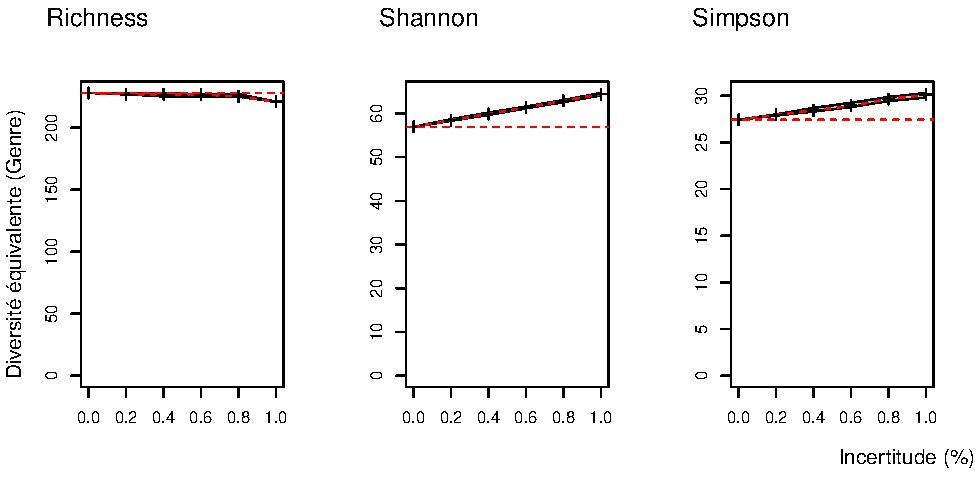
\includegraphics[width=0.6\linewidth]{MyBook_files/figure-latex/FigTreesGenus-1} 

}

\caption{Profil de biais pour les diversité de Richesse, Shannon et Simpson au niveau genre le long d'un gradient d'indétermination correspondant au pourcentage d'individus identifiés uniquement par leur nom vernaculaire. Les profils de biais représentent la moyenne et les quantiles 0.025 et 0.975 de la distribution des diversités obtenues pour 100 simulations de tirage aléatoire et de propagation des incertitudes.}\label{fig:FigTreesGenus}
\end{figure*}

\subsection{Cas particulier de
Paracou}\label{cas-particulier-de-paracou}

L'histoire de détermination botanique des parcelles de Paracou implique
une grande variabilité du degré d'indétermination au cours du temps et
des différences significatives entres les parcelles. Aujourd'hui tandis
que les parcelles contrôle et du traitement 3 sont bien déterminées,
moins de 5\% des arbres 'ne sont identifiés que par un nom
vernaculaire'ont pas d'identification botanique, d'autres parcelles du
traitement 1 ou 2 sont encore mal déterminées et pour certaines plus de
30\% des arbres n'ont pas d'identification botanique.

Jusqu'à présent le biais des estimateurs de diversité reste à resoudre,
en revanche il est possible de pallier ces différences de détermination
en considérant la compositon et la diversité des parcelles au niveau du
genre plutôt qu'au niveau de l'espèce.

\chapter{Article 2: trajectoires de diversité des
parcelles}\label{article-2-trajectoires-de-diversite-des-parcelles}

Nous proposons ici d'étudier les trajectoires de diversité et de
composition taxonomique et fonctionnelle en forêt tropicale sur 30
années après perturbation pour identifier les processus écologiques
déterminants la dynamique des communautés. Nous avons plus
particulièrement analysé les trajectoires taxonomiques et fonctionnelles
de composition, de richesse et d'équitabilitéet de redondance
fonctionnelle, en considérant 7 traits fonctionnels représentatifs de
lécologie des espèces.

Ces trajectoires ont montré la restoration taxonomique des communautés
initiales d'une part, traduisant le maintien de leurs différences de
composition, et d'autre partdes trajectoires fonctionnelles communes
dans l'espace des traits déterminées par l'intensité de la perturbation,
validant la théorie des perturbations intermédiaires Les trajectoires
après perturbations ont cependant démontré un décalage entre les
trajectoires taxonomiques et fonctionnelles traduisant une récupération
fonctionnelle rapide mais une récupération taxonomique des espèces rares
inféodées aux peuplements matures ralentie par l'exclusion compétitive
pour la lumière avec les espèces dominantes. Si la théorie des
perturbations intermédiaires s'est avérée prédire correctement les
trajectoires fonctionnelles, elle ne représentait que médiocrement les
trajectoires taxonomiques troublées par la réorganisation de la
redondance fonctionnelle adns l'espace des traits.

Bien que le fonctionnement des communautés soit restoré 30 ans après
perturbation la récupération des espèces rares reste inachevée, altérant
la structure taxonomique et la redondance fonctionnelle de la
communauté. Ces résultats soulignent d'une part seuls des cycles de
régénération longs de plusieurs décennies permettent la récupération
complète de la communauté et préviennent la perte d'espèces, et d'autre
part ils interrogent sur la résilience des peuplement saprès plusieurs
perturbations.

\chapter{Article 3: Analyse du recrutement, support de la trajectoire
des
communautés}\label{article-3-analyse-du-recrutement-support-de-la-trajectoire-des-communautes}

La littérature récente en écologie tropicale a démontré l'implication de
processus déterministes et stochastiques dans la dynamique des
communautés mais leur signature structurelle sont difficilement
distinguables \autocites{Mouquet2003}{Chave2004}. Nous proposons ici de
clarifier le rôle des processus écologiques régissant la réponse des
communautés en distinguant la trajectoire du recrutement de celle de la
communauté entière. Ces trajectoires de recrutement permettent d'une
part de distinguer les processus stochastiques et déterministes qui les
régissent, de spécifier les processus de compétition impliqués et de
déterminer la durée et l'intégralité de la résilience des communautés et
de leur fonctionnement.

Nous avons pour cela suivi pendant 30 ans les trajectoires de diversité
et de composition du recrutement dans 70ha de forêts néotropicale
Amazonienne après un gradient de perturbation (de 15 à 60\% de la
biomasse prélevée). Nous avons analysé et comparé à des modèles nuls les
trajectoires de diversité et d'équitabilité taxonomique, de
renouvellement des espèces recrutées par rapport à la communauté
initiale avant perturbation, et de la diversité fonctionnelle (indice de
Rao) de 7 trais fonctionnels majeurs des feuilles, du bois et d'histoire
de vie.

Nous avons identifié trois phases de recrutement après perturbation,
définies par l'équilibre entre les processus déterministes et
stochastiques impliqués. Dans un premier temps les trajectoires sont
portées par la croissance de juvéniles recrutés aléatoirement dans la
communauté d'avant exploitation. Dans un deuxième temps les trajectoires
reposent sur les ``recrutés vrais'' issus de la banque de graines et
tributaires de processus d'exclusion pour la lumière favorisant les
espèces héliophiles à croissance rapide. La troisième et dernière phase
des trajectoires correspond au retour progressif vers un recrutement
aléatoire restorant la structure, la composition taxonomique et le
fonctionnement de la communauté initiale. Si le fontionnement du
recrutement a été rapidement retrouvé, la restoration taxonomique s'est
montrée longue, ce qui interroge l'intégralité de la résilience et
malgré la réelle restoration de la diversité et de la composition
initiale, Les différentes trajectoires ont par ailleurs confirmé une
restoration de la diversité fonctionnelle rapide mais plus lente de la
composition et de la diversité taxonomiques.

La trajectoire des communautés après perturbation résulte de la
combinaison des processus stochastiques, majeurs avant perturbation et
progressivement restorés par la suite, et de processus déterministes
d'exclusion compétitive favorisant les espèces héliophiles et à
croissance rapide. La résilience de la composition et la diversité
taxonomiques et fonctionnelles du recrutement a été confirmée mais
longue de plusieurs décennies, et confirme le risque de trajectoires
différentes dans le cas de perturbations répétées.

\chapter{Conclusion et perspectives}\label{conclusion-et-perspectives}


% Bibliography
%%%%%%%%%%%%%%%%%%%%%%%%%%%%%%%%%%%%%%%%%%%%%%%%%%%%%%%%%%

\backmatter
\SmallMargins

%
\printbibliography


% Tables (of tables, of figures)
%%%%%%%%%%%%%%%%%%%%%%%%%%%%%%%%%%%%%%%%%%%%%%%%%%%%%%%%%%




% After-body (LaTeX code inclusion)
%%%%%%%%%%%%%%%%%%%%%%%%%%%%%%%%%%%%%%%%%%%%%%%%%%%%%%%%%%



% Back cover
%%%%%%%%%%%%%%%%%%%%%%%%%%%%%%%%%%%%%%%%%%%%%%%%%%%%%%%%%%%

% Even page, small margins, no running head, no page number.
\evenpage
\SmallMargins
\thispagestyle{empty}

\begin{normalsize}

\begin{description}

\selectlanguage{french}
\item[Résumé:]
A venir

\selectlanguage{french}
\item[Mots clés :]
Biodiversite, Forets Neotropicales, Perturbation, Ecologie des Communautes, Trajectoires dynamiques, Resilience.
~\\

\selectlanguage{english}
\item[Abstract:]
To be coming

\selectlanguage{english}
\item[Keywords:]
Biodiversity, Neotropical forests, Perturbation, Communities Ecology, Dynamic trajectories, Resilience.

\end{description}

\end{normalsize}

\vspace*{\fill}
\centering\includegraphics[width=.3\textwidth]{images/Logo-Lab}
\end{document}
